% !TEX root = master_thesis.tex
\chapter{Extraction of the beam asymmetries $\Sigma_{\eta}$ and $\Sigma_{\eta'}$}
The beam asymmetry $\Sigma$ is observable when a linearly polarized photon beam and unpolarized liquid hydrogen target are employed. The polarized cross section $\frac{\text{d}\sigma}{\text{d}\Omega}_\text{pol}$ is not symmetric in the azimuthal angle $\phi$ anymore as opposed to the unpolarized cross section $\frac{\text{d}\sigma}{\text{d}\Omega}_0$. It is rather modulated by a cosine dependence which scales with the polarization observable $\Sigma$ and the (linear) beam polarization $p_\gamma$, see equation \eqref{eq:asym} \cite{san}.
\begin{equation}
	\frac{\text{d}\sigma}{\text{d}\Omega}_\text{pol}\left(E_\gamma,\cos\theta,\phi\right)=\frac{\text{d}\sigma}{\text{d}\Omega}_0\left(E_\gamma,\cos\theta\right)\cdot\left[1-p_\gamma\Sigma\left(E_\gamma,\cos\theta\right)\cos\left(2\varphi\right)\right]
	\label{eq:asym}
\end{equation}
Since the incident photon beam is polarized, photon momentum $\vec{k}$ and polarization $\vec{\epsilon}$ span a plane which is referred to as the beam polarization plane. This plane is tilted by the angle $\varphi$ with respect to the reaction plane which is defined by the final state momenta. Naturally, this plane builds the angle $\phi$ in the laboratory system. At the same time the angle of the beam polarization plane in the same reference frame is defined as $\alpha$. It holds 
\begin{equation}
	\varphi=\alpha-\phi.
\end{equation} Figure \ref{fig:angles} illustrates definitions of all angles and planes. 
 \begin{figure}[htbp]
	\centering
	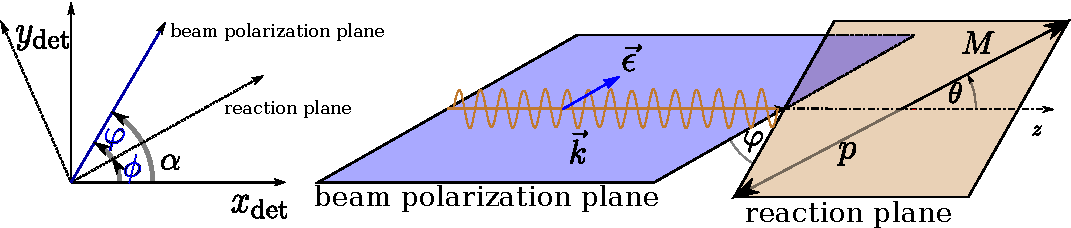
\includegraphics[width=\linewidth]{../DPG2022/figs/angles.pdf}
	\caption{Left: Definition of angles $\alpha,\phi,\varphi$. Right: Photon momentum $\vec{k}$ and polarization  $\vec{\epsilon}$ define the beam polarization plane while the reaction plane is defined by the recoil proton $p$ and produced meson $M$.}
	\label{fig:angles}
\end{figure} 
Theoretically the beam asymmetry can be determined by a measurement of the cross section and a fit using equation \eqref{eq:asym}. However, when calculating polarized cross sections, it is important to have good control over flux normalization and detector acceptance in three dimensions $(E_\gamma,\cos\theta,\phi)$. To avoid this, the measurement of asymmetries can be used to access the polarization observable $\Sigma$ instead. Particularly, data is taken for two distinct orthogonal polarization settings corresponding to $\alpha=\pm\SI{45}{\degree}$.

This chapter will illustrate the process of determining the beam asymmetry for $\eta$ and $\eta'$ photoproduction. The published results of $\Sigma_{\eta}$ \cite{farahphd,eta} are used to check the accuracy and functionality of employed bayesian methods. Bayesian methods, as well as traditional frequentist approaches are used afterwards to extract new results for $\Sigma_{\eta'}$. First, the used methods will be presented and subsequently their application for each final state, respectively.
\section{Methods}
\label{sec:meth}
The beam asymmetry has to be determined via fits to $\phi$ distributions obtained from data. These are performed as either binned or unbinned fits. Both methods allow the application of Bayesian methods as will be discussed in the following. Additionally the advantages and disadvantages off all methods are compared.
\subsection{Event yield asymmetries}
Measurements were made in two distinct polarization settings $\alpha=\pm\SI{45}{\degree}=\alpha^{\bot/\parallel}$. Thus, the polarized cross sections for both settings are given by\footnote{The dependencies of polarized and unpolarized cross sections as well as the beam asymmetry like in equation \eqref{eq:asym} are implied}
\begin{equation}
	\frac{\text{d}\sigma}{\text{d}\Omega}_\text{pol}^\parallel=\frac{\text{d}\sigma}{\text{d}\Omega}_0\cdot\left[1-p_\gamma^\parallel\Sigma\cos\left(2\left(\alpha^\parallel-\phi\right)\right)\right]
	\label{eq:polcs0}
\end{equation}
and 
\begin{align}
	\frac{\text{d}\sigma}{\text{d}\Omega}_\text{pol}^\bot&=\frac{\text{d}\sigma}{\text{d}\Omega}_0\cdot\left[1-p_\gamma^\bot\Sigma\cos\left(2\left(\alpha^\bot-\phi\right)\right)\right]\\
	&=\frac{\text{d}\sigma}{\text{d}\Omega}_0\cdot\left[1+p_\gamma^\bot\Sigma\cos\left(2\left(\alpha^\parallel-\phi\right)\right)\right].\label{eq:polcs}
\end{align}
Note that equation \eqref{eq:polcs} holds, because 
\begin{align*}
	\alpha^\bot=\alpha^\parallel+\pi/2 &&\text{and}&&\cos x = -1\cdot\cos(x+\pi).
\end{align*}
Consider now taking the difference of equations \eqref{eq:polcs0} and \eqref{eq:polcs}
\begin{equation}
	\frac{\text{d}\sigma}{\text{d}\Omega}_\text{pol}^\bot-\frac{\text{d}\sigma}{\text{d}\Omega}_\text{pol}^\parallel=\frac{\text{d}\sigma}{\text{d}\Omega}_0\cdot\left(p_\gamma^\bot+p_\gamma^\parallel\right)\Sigma\cos\left(2\left(\alpha^\parallel-\phi\right)\right).
\end{equation}
One can further eliminate the unpolarized cross section from this equation by dividing by the polarization weighted sum of equations \eqref{eq:polcs0} and \eqref{eq:polcs}
\begin{equation}
	\alpha\cdot\frac{\text{d}\sigma}{\text{d}\Omega}_\text{pol}^\parallel+\beta\cdot\frac{\text{d}\sigma}{\text{d}\Omega}_\text{pol}^\bot=\frac{\text{d}\sigma}{\text{d}\Omega}_0\cdot\left[\alpha+\beta-\left(\alpha p_\gamma^\parallel-\beta p_\gamma^\bot\right)\Sigma\cos\left(2\left(\alpha^\bot-\phi\right)\right)\right]\overset{!}{=}2\frac{\text{d}\sigma}{\text{d}\Omega}_0.
\end{equation}
Since $$\frac{\text{d}}{\text{d}\phi}\frac{\text{d}\sigma}{\text{d}\Omega}_0\overset{!}{=}0\forall\phi$$ it holds \begin{align}
	\alpha p_\gamma^\parallel-\beta p_\gamma^\bot \overset{!}{=}0 && \alpha+\beta\overset{!}{=}2,
\end{align}
such that
\begin{align}
	\alpha =\frac{2p_\gamma^\parallel}{p_\gamma^\bot+p_\gamma^\parallel} && \beta=\frac{2p_\gamma^\bot}{p_\gamma^\bot+p_\gamma^\parallel}.
	\label{eq:alphabeta}
\end{align}
The beam asymmetry $\Sigma$ is thus accessible via the asymmetry \begin{equation}
	A(\phi)=\frac{\frac{\text{d}\sigma}{\text{d}\Omega}_\text{pol}^\bot-\frac{\text{d}\sigma}{\text{d}\Omega}_\text{pol}^\parallel}{p_\gamma^\parallel\frac{\text{d}\sigma}{\text{d}\Omega}_\text{pol}^\bot+p_\gamma^\bot\frac{\text{d}\sigma}{\text{d}\Omega}_\text{pol}^\parallel}=\Sigma\cos\left(2\left(\alpha^\parallel-\phi\right)\right).
	\label{eq:asymfit}
\end{equation}
At this point one can now make use of the fact that in any scattering reaction the number of events $N$ is given by the product of luminosity $L$ and total cross section $\sigma$ $$N=L\cdot\sigma=\Phi\cdot N_t\cdot\frac{\text{d}\sigma}{\text{d}\Omega}\cdot\Delta\Omega,$$
where $\Phi$ is the beam flux, $N_t$ the number of target particles and $\Delta\Omega$ is the solid angle covered by the detector. Substituting this in equation \eqref{eq:asymfit} one can build the asymmetry $A(\phi)$ using only the (flux-)normalized event yields $\tilde{N}^{\parallel/\bot}\left(E_\gamma,\cos\theta,\phi\right)$\footnote{again, arguments $\left(E_\gamma,\cos\theta,\phi\right)$ are implied.}
\begin{equation}
	A(\phi)=\frac{\tilde{N}^\bot-\tilde{N}^\parallel}{p_\gamma^\parallel\tilde{N}^\bot+p_\gamma^\bot\tilde{N}^\parallel}=\Sigma\cos\left(2\left(\alpha^\parallel-\phi\right)\right).
	\label{eq:evyieldasym}
\end{equation}
Alternatively, the event yields $N$ can also be normalized by integrating over the total azimuthal angle range in each bin of $(E_\gamma,\cos\theta)$. This normalization technique has been used in reference \cite{farahphd} and will also be used in this work. Using appropriate additional binning in $\phi$ the asymmetry can be build for all kinematic bins and the beam asymmetry then be extracted via a one-Parameter fit. The statistical errors for $A(\phi)$ are given by \textsc{Gaussian} error propagation (see \ref{sec:stat_err})
\subsubsection{Frequentist}
The traditional approach to this fitting problem is a $\chi^2$ fit. The test-statistic.
\subsubsection{Bayesian}
\subsection{Event based fit}
\subsubsection{Frequentist}
\subsubsection{Bayesian}
\section{Determination of $\Sigma_{\eta}$ using Bayesian statistics}
\subsection{Event yield asymmetries}
\subsubsection{Application of method to toy Monte Carlo data}
\subsubsection{Application of method to data}
\subsection{Event based fit}
\subsubsection{Application of method to toy Monte Carlo data}
\subsubsection{Application of method to data}
\subsection{Discussion}
\section{Determination of $\Sigma_{\eta'}$}
\subsection{Application of event based fit to toy Monte Carlo data}
\subsection{Application of event based fit to data}
\subsection{Systematic Error}